\section{Planning}
\label{ann:planning}

Pour réaliser notre planning, nous avons utilisé le logiciel \textsc{GanttProject}
qui permet d'assigner des tâches sur une certaine période à différents membres.
Les couleurs nous permettent également de rassembler les tâches en différents 
sous-groupes, on retrouvera par exemple la couleur rouge pour les rapports finaux.
On peut voir dans la Figure~\ref{fig:planning_gant} que cela nous permet également
d'avoir une vision générale des tâches qu'il reste à réaliser.

\begin{figure}[h]
  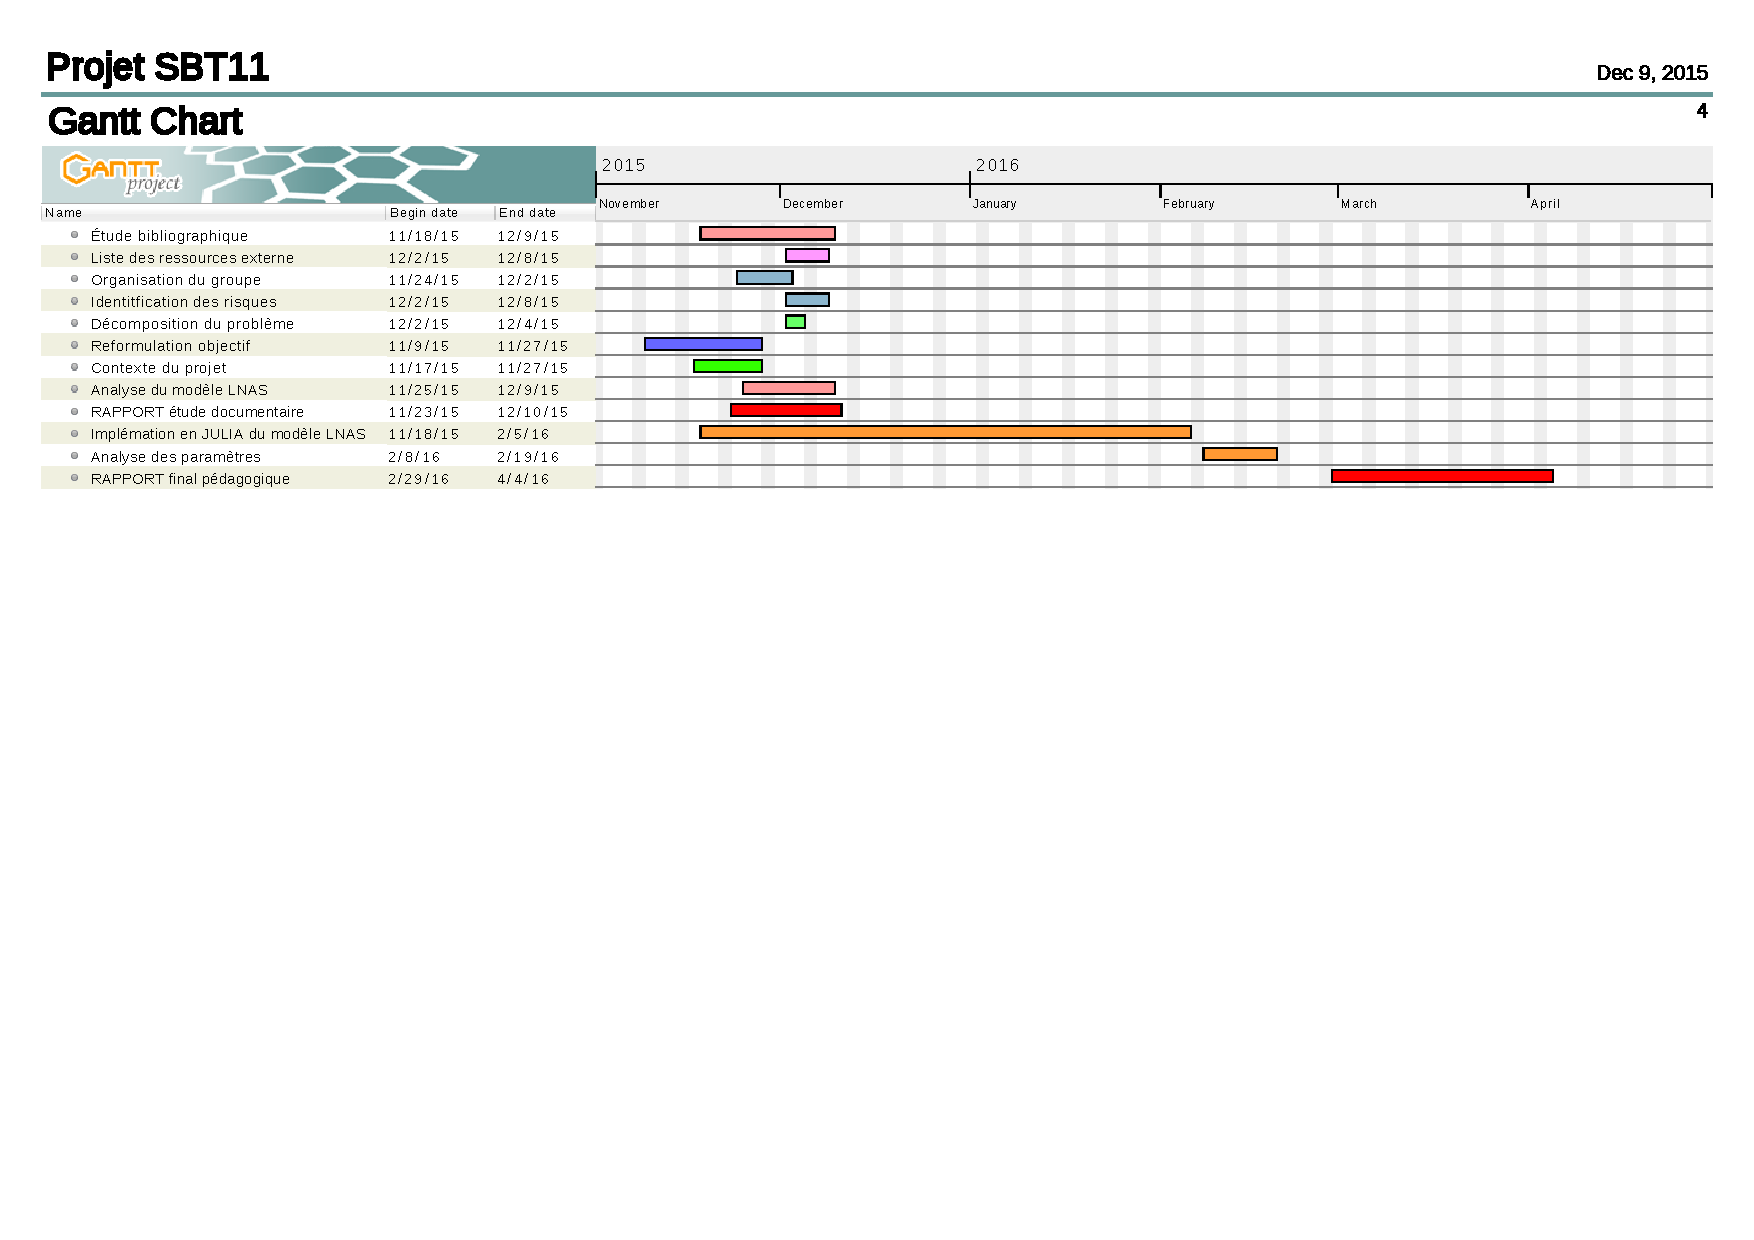
\includegraphics[scale=0.51]{./annexes/planning_gant.pdf}
  \caption{Planning \textsc{Gantt} des différentes tâches.}
  \label{fig:planning_gant}
\end{figure}